% Font size, paper type
\documentclass[12pt]{article}
% Aesthetic margins
\usepackage[margin=1in]{geometry}
% Core math packages,
% Mathtools loads amsmath, and amsmath gives basic math symbs
% Amsfonts & amssymb are misc. symbols you might need
\usepackage{mathtools, amsfonts, amssymb}
% Links in a pdf
\usepackage{hyperref}
% Use in pictures, graphs, and figures
\usepackage{graphicx}
% Header package
\usepackage{fancyhdr}
% Underlining with line breaks
\usepackage{ulem}
% Adjust accordingly given warning messages
\setlength{\headheight}{15pt}
% So we can more easily format text with pictures
\usepackage{float}

% Sets footer
\pagestyle{fancy}
% Removes default footer style
\fancyhf{}

\rhead{
  Shengdong Li
  Calc 3
}

\rfoot{
  Page \thepage
}

% Makes links look more appealling
\hypersetup{
    colorlinks=true,
    linkcolor=blue,
    filecolor=magenta,      
    urlcolor=cyan,
}

% \usepackage{indentfirst}

\begin{document}
\title{Initial Post: Epicycloid}
\author{by Shengdong Li}
\date{15 December 2020}
\maketitle

\begin{align*}
  x(t) & =\left(a+b\right)\cos t-b\cos\left(\left(\frac{a}{b}+1\right)t\right) \\
  y(t) & =\left(a+b\right)\sin t-b\sin\left(\left(\frac{a}{b}+1\right)t\right) \\
\end{align*}

\section{Observations}
(See GIF below)

Oftentimes, the graph takes the shape of a flower, with constants affecting the size of the flower and petals

For example, if we set $T$ to a small value, say $t=3$, keep $a=1$, and modify the $b$ value between $0$ and $1$, we can see that the 'petals' get their size proportional to the value of $b$. The size of the entire flower is also proportional to $b$, but only slightly.

Keeping $b=0.1$, and modifying $a$, we can now clearly see that the size of the entire flower is much more sensitive and proportional to $a$, but the size of the 'petals' are still generally the same.
\section{Fixed Equation}
\begin{align*}
  \intertext{For my fixed equation, I decided to set $a=5$ and $b=2$ which, as t gets to $4\pi$, turns into a nice cherry blossom graph.}
  \intertext{This gave me an $x(t)$ and $y(t)$ of }
  x(t)            & =7\cos t-2\cos\left(\frac{7}{2}t\right)                                                       \\
  y(t)            & =7\sin t-2\sin\left(\frac{7}{2}t\right)                                                       \\
  \intertext{And thus a a $c(t)$ of}
  c\left(t\right) & =\left(7\cos t-2\cos\left(\frac{7}{2}t\right),\ 7\sin t-2\sin\left(\frac{7}{2}t\right)\right) \\
\end{align*}
\begin{figure}[H]
  \begin{center}
    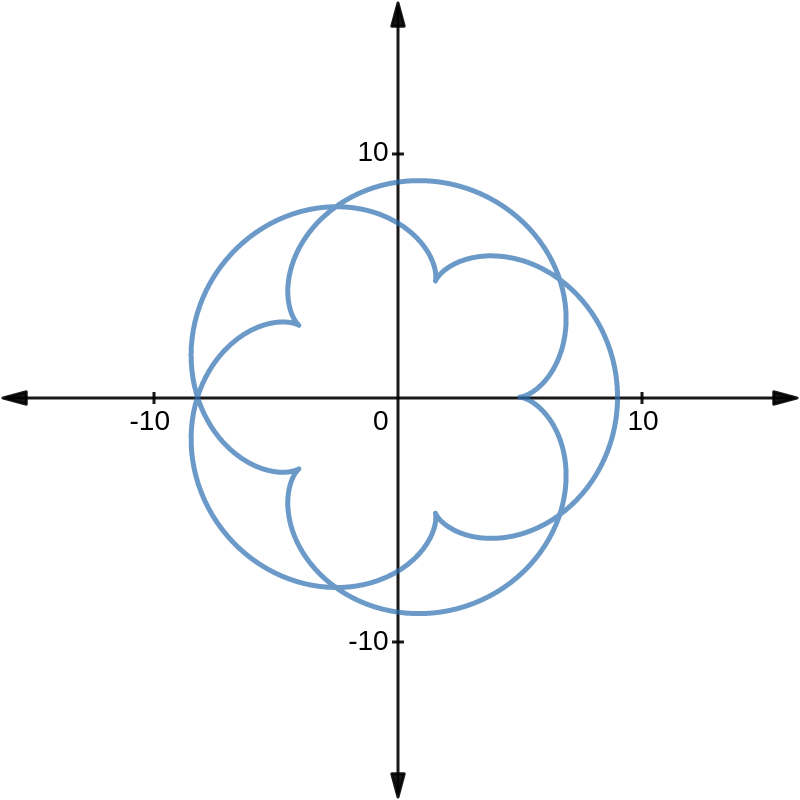
\includegraphics[scale=.3]{base.png}
    \caption{\textit{Graph of equation with fixed variables.} Desmos link \href{https://www.desmos.com/calculator/lz7drdxhpy}{\textcolor{blue}{here}}}
  \end{center}
\end{figure}
\section{Three Points}
\begin{align}
  \intertext{Since my figure is complete at $4\pi$, I decided to choose $t$ values in denominations of $\pi$. My three $t$s were then $t={\frac{\pi}{2},\pi, 2\pi}$}
  \intertext{Plugging in the values of $t$ as follows:}
  \intertext{$t=\frac{\pi}{2}$}
  x\left(\frac{\pi}{2}\right) & =7\cos\left(\frac{\pi}{2}\right)-2\cos\left(\frac{7}{2}\left(\frac{\pi}{2}\right)\right) \\
                              & =-2\cos\left(\frac{7}{4}\pi\right)                                                       \\
                              & =-\sqrt{2}                                                                               \\
  y\left(\frac{\pi}{2}\right) & =7\sin\left(\frac{\pi}{2}\right)-2\sin\left(\frac{7}{2}\left(\frac{\pi}{2}\right)\right) \\
                              & =7-2\sin\left(\frac{7}{4}\pi\right)                                                      \\
                              & =7+\sqrt{2}                                                                              \\
  c\left(\frac{\pi}{2}\right) & =\left(-\sqrt{2},7+\sqrt{2}\right)                                                       \\
  \intertext{$t=\pi$}
  x\left(\pi\right)           & =7\cos\left(\pi\right)-2\cos\left(\frac{7}{2}\left(\pi\right)\right)                     \\
                              & =-7-2\cos\left(\frac{3}{2}\pi\right)                                                     \\
                              & =-7                                                                                      \\
  y\left(\pi\right)           & =\ 7\sin\left(\pi\right)-2\sin\left(\frac{3}{2}\left(\pi\right)\right)                   \\
                              & =0-2\sin\left(\frac{3}{2}\pi\right)                                                      \\
                              & =2                                                                                       \\
  c\left(\pi\right)           & =\left(-7,2\right)                                                                       \\
  \intertext{$t=2\pi$}
  x\left(2\pi\right)          & =7\cos\left(2\pi\right)-2\cos\left(\frac{7}{2}\left(2\pi\right)\right)                   \\
                              & =7-2\cos\left(\pi\right)                                                                 \\
                              & =9                                                                                       \\
  y\left(2\pi\right)          & =7\sin\left(2\pi\right)-2\sin\left(\frac{3}{2}\left(2\pi\right)\right)                   \\
                              & =0-2\sin\left(\pi\right)                                                                 \\
                              & =0                                                                                       \\
  c\left(2\pi\right)          & =\left(9,0\right)                                                                        \\
\end{align}
To summarize, the points of interests are
\begin{align*}
  c\left(\frac{\pi}{2}\right) & = \left(-\sqrt{2},7+\sqrt{2}\right) \\
  c\left(\pi\right)           & = \left(-7,2\right)                 \\
  c\left(2\pi\right)          & = \left(9, 0\right)
\end{align*}
\section{Tangent Line}
\begin{align}
  \intertext{To find the tangent line, we just need to find the equation for the first derivative, and plugin our points to get the slope, which we can then use to plugin to point-slope}
  \intertext{First recall the formula for the first derivative of parametric equations }
  c'\left(t\right)          & =\frac{y'\left(t\right)}{x'\left(t\right)}                                                                                                                                           \\
  \intertext{Calculate $y'(t)$}
  y\left(t\right)           & =7\sin t-2\sin\left(\frac{7}{2}t\right)                                                                                                                                              \\
  y'\left(t\right)          & =7\cos t-2\cos\left(\frac{7}{2}t\right)\cdot\frac{7}{2}                                                                                                                              \\
                            & =7\cos t-7\cos\left(\frac{7}{2}t\right)                                                                                                                                              \\
  \intertext{Calculate $x'(t)$}
  x\left(t\right)           & =7\cos t-2\cos\left(\frac{7}{2}t\right)                                                                                                                                              \\
  x'\left(t\right)          & =-7\sin t-\left(-2\sin\left(\frac{7}{2}t\right)\cdot\frac{7}{2}\right)                                                                                                               \\
                            & =7\sin\left(\frac{7}{2}t\right)-7\sin t                                                                                                                                              \\
  \intertext{Plugin to derivative formula}
  c'\left(t\right)          & =\frac{7\cos t-7\cos\left(\frac{7}{2}t\right)}{7\sin\left(\frac{7}{2}t\right)-7\sin t}                                                                                               \\
                            & =\frac{\cos t-\cos\left(\frac{7}{2}t\right)}{\sin\left(\frac{7}{2}t\right)-\sin t}                                                                                                   \\
  \intertext{Tangent line for $(-\sqrt{2},7+\sqrt{2})$ @ $t=\frac{\pi}{2}$}
  m                         & =\frac{\cos\left(\frac{\pi}{2}\right)-\cos\left(\frac{7}{2}\left(\frac{\pi}{2}\right)\right)}{\sin\left(\frac{7}{2}\left(\frac{\pi}{2}\right)\right)-\sin\left(\frac{\pi}{2}\right)} \\
                            & =\frac{0-\frac{\sqrt{2}}{2}}{-\frac{\sqrt{2}}{2}-1}                                                                                                                                  \\
                            & =\frac{\frac{\sqrt{2}}{2}}{\frac{\sqrt{2}}{2}+1}\cdot\frac{\frac{\sqrt{2}}{2}-1}{\frac{\sqrt{2}}{2}-1}                                                                               \\
                            & =\frac{\frac{1}{2}-\frac{\sqrt{2}}{2}}{-\frac{1}{2}}                                                                                                                                 \\
                            & =\sqrt{2}-1                                                                                                                                                                          \\
  \intertext{Now we can plug the slope and points into the point slope formula}
  y-\left(7+\sqrt{2}\right) & =\left(\sqrt{2}-1\right)\left(x-\left(-\sqrt{2}\right)\right)                                                                                                                        \\
  y                         & =\left(\sqrt{2}-1\right)\left(x+\sqrt{2}\right)+\left(7+\sqrt{2}\right)                                                                                                              \\
  y                         & =x\sqrt{2}+2-x-\sqrt{2}+7+\sqrt{2}                                                                                                                                                   \\
  y                         & =\left(\sqrt{2}-1\right)x+9                                                                                                                                                          \\
  \intertext{Tangent line for $(-7,2)$ @ $t=\pi$}
  m                         & =\frac{\cos\left(\pi\right)-\cos\left(\frac{7}{2}\left(\pi\right)\right)}{\sin\left(\frac{7}{2}\left(\pi\right)\right)-\sin\left(\pi\right)}                                         \\
                            & =\frac{-1-0}{-1-0}                                                                                                                                                                   \\
                            & =1                                                                                                                                                                                   \\
  \intertext{Now we can plug the slope and points into the point slope formula}
  y-2                       & =x+7                                                                                                                                                                                 \\
  y                         & =x+9                                                                                                                                                                                 \\
  \intertext{Tangent line for $(9, 0)$ @ $t=2\pi$}
  m                         & =\frac{\cos\left(2\pi\right)-\cos\left(\frac{7}{2}\left(2\pi\right)\right)}{\sin\left(\frac{7}{2}\left(2\pi\right)\right)-\sin\left(2\pi\right)}                                     \\
                            & =\frac{1-\left(-1\right)}{0-0}                                                                                                                                                       \\
                            & =\frac{2}{0}                                                                                                                                                                         \\
                            & =DNE                                                                                                                                                                                 \\
  \intertext{Since the slope of the line does not exist, but by inspection of the graph at $(9, 0)$ we can see that the function is continuous and has no sharp bends, we can safely say that there is a vertical line at}
  x                         & =9                                                                                                                                                                                   \\
\end{align}
To summarize, the tangent lines are as follows
\begin{align}
  y & =\left(\sqrt{2}-1\right)x+9 \\
  y & =x+9                        \\
  x & =9
\end{align}
\begin{figure}[H]
  \begin{center}
    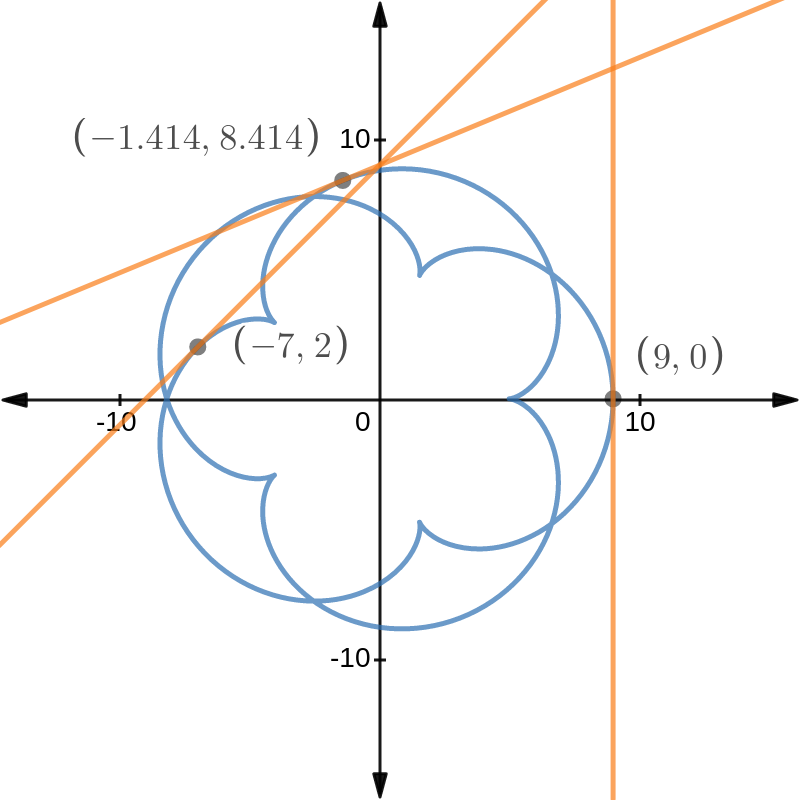
\includegraphics[scale=.3]{after.png}
    \caption{\textit{Graph of parametric with points and tangent lines.} Desmos link \href{https://www.desmos.com/calculator/lz7drdxhpy}{\textcolor{blue}{here}}}
  \end{center}
\end{figure}
\section{Second Derivative}
\begin{align}
  \intertext{From finding the slope of tangent lines, we already have $x'(x)$ and $y'(x)$, so we only need $y''(x)$ $x''(x)$ }
  y''\left(x\right) & =\left(7\cos t-7\cos\left(\frac{7}{2}t\right)\right)\frac{d}{dx} \\
                    & =-7\sin t+\frac{49}{2}\sin\left(\frac{7}{2}t\right)              \\
                    & =\frac{49}{2}\sin\left(\frac{7}{2}t\right)-7\sin t               \\
  x''\left(x\right) & =\left(7\sin\left(\frac{7}{2}t\right)-7\sin t\right)\frac{d}{dx} \\
                    & =\frac{49}{2}\cos\left(\frac{7}{2}t\right)-7\cos t
\end{align}
\begin{align}
  \intertext{Now we can plugin our first and second derivatives $x'(t)$, $x''(t)$, $y'(t)$, and $y''(t)$}
  c''\left(t\right) & =\frac{\left(7\sin\left(\frac{7}{2}t\right)-7\sin t\right)\left(\frac{49}{2}\sin\left(\frac{7}{2}t\right)-7\sin t\right)-\left(7\cos t-7\cos\left(\frac{7}{2}t\right)\right)\left(\frac{49}{2}\cos\left(\frac{7}{2}t\right)-7\cos t\right)}{\left(7\sin\left(\frac{7}{2}t\right)-7\sin t\right)^{3}}         \\
  \intertext{First we can take out some coefficients}
                    & =\frac{7\left(\sin\left(\frac{7}{2}t\right)-\sin t\right)7\left(\frac{7}{2}\sin\left(\frac{7}{2}t\right)-\sin t\right)+7\left(\cos\left(\frac{7}{2}t\right)-\cos t\right)7\left(\frac{7}{2}\cos\left(\frac{7}{2}t\right)-\cos t\right)}{\left(7\left(\sin\left(\frac{7}{2}t\right)-\sin t\right)\right)^{3}} \\
                    & =\frac{\left(\sin\left(\frac{7}{2}t\right)-\sin t\right)\left(\frac{7}{2}\sin\left(\frac{7}{2}t\right)-\sin t\right)+\left(\cos\left(\frac{7}{2}t\right)-\cos t\right)\left(\frac{7}{2}\cos\left(\frac{7}{2}t\right)-\cos t\right)}{7\left(\sin\left(\frac{7}{2}t\right)-\sin t\right)^{3}}                  \\
                    & =\frac{\left(\sin\left(\frac{7}{2}t\right)-\sin t\right)\left(\frac{7}{2}\sin\left(\frac{7}{2}t\right)-\sin t\right)+\left(\cos\left(\frac{7}{2}t\right)-\cos t\right)\left(\frac{7}{2}\cos\left(\frac{7}{2}t\right)-\cos t\right)}{7\left(\sin\left(\frac{7}{2}t\right)-\sin t\right)^{3}}                  \\
  \intertext{Then the only course here I found was to distribute}
                    & =\frac{\frac{7}{2}\sin\left(\frac{7}{2}t\right)^{2}-\frac{9}{2}\sin\left(\frac{7}{2}t\right)\sin t+\sin^{2}t+\frac{7}{2}\cos\left(\frac{7}{2}t\right)^{2}-\frac{9}{2}\cos\left(\frac{7}{2}t\right)\cos t+\cos^{2}t}{7\left(\sin\left(\frac{7}{2}t\right)-\sin t\right)^{3}}                                  \\
                    & =\frac{\frac{7}{2}\sin\left(\frac{7}{2}t\right)^{2}-\frac{9}{2}\sin\left(\frac{7}{2}t\right)\sin t+\frac{7}{2}\cos\left(\frac{7}{2}t\right)^{2}-\frac{9}{2}\cos\left(\frac{7}{2}t\right)\cos t+1}{7\left(\sin\left(\frac{7}{2}t\right)-\sin t\right)^{3}}                                                    \\
  \intertext{Recall the angle identity here that $\sin^2(x) = \frac{1-\cos2x}{2}$, and $\cos^2(x) = \frac{1+\cos2x}{2}$}
                    & =\frac{\frac{7}{2}\left(\frac{1-\cos2t}{2}\right)-\frac{9}{2}\sin\left(\frac{7}{2}t\right)\sin t+\frac{7}{2}\left(\frac{1+\cos2t}{2}\right)-\frac{9}{2}\cos\left(\frac{7}{2}t\right)\cos t+1}{7\left(\sin\left(\frac{7}{2}t\right)-\sin t\right)^{3}}                                                        \\
  \intertext{Expand the substitution}
                    & =\frac{\frac{7}{4}-\frac{7}{4}\cos2t-\frac{9}{2}\sin\left(\frac{7}{2}t\right)\sin t+\frac{7}{4}+\frac{7}{4}\cos2t-\frac{9}{2}\cos\left(\frac{7}{2}t\right)\cos t+1}{7\left(\sin\left(\frac{7}{2}t\right)-\sin t\right)^{3}}
\end{align}
\begin{align}
  \intertext{The $\cos(2t)$s cancel}
                                                  & =\frac{\frac{9}{2}-\frac{9}{2}\sin\left(\frac{7}{2}t\right)\sin t-\frac{9}{2}\cos\left(\frac{7}{2}t\right)\cos t}{7\left(\sin\left(\frac{7}{2}t\right)-\sin t\right)^{3}}                                                                        \\
  \intertext{Then we can factor out the coefficients }
                                                  & =\frac{9\left(1-\sin\left(\frac{7}{2}t\right)\sin t-\cos\left(\frac{7}{2}t\right)\cos t\right)}{14\left(\sin\left(\frac{7}{2}t\right)-\sin t\right)^{3}}                                                                                         \\
  \intertext{Yet some other trig identities we can use here are the product and sum formulas}
  \cos\left(a\right)\cos\left(b\right)            & =\frac{1}{2}\left(\cos\left(a+b\right)+\cos\left(a-b\right)\right)                                                                                                                                                                               \\
  \cos\left(\frac{7}{2}t\right)\cos\left(t\right) & =\frac{1}{2}\left(\cos\left(\frac{9}{2}t\right)+\cos\left(\frac{5}{2}t\right)\right)                                                                                                                                                             \\
  \sin\left(a\right)\sin\left(b\right)            & =\frac{1}{2}\left(\cos\left(a-b\right)-\cos\left(a+b\right)\right)                                                                                                                                                                               \\
  \sin\left(\frac{7}{2}t\right)\sin\left(t\right) & =\frac{1}{2}\left(\cos\left(\frac{5}{2}t\right)-\cos\left(\frac{9}{2}t\right)\right)                                                                                                                                                             \\
                                                  & =\frac{9\left(1-\frac{\cos\left(\frac{5}{2}t\right)}{2}+\frac{\cos\left(\frac{9}{2}t\right)}{2}-\frac{\cos\left(\frac{9}{2}t\right)}{2}-\frac{\cos\left(\frac{5}{2}t\right)}{2}\right)}{14\left(\sin\left(\frac{7}{2}t\right)-\sin t\right)^{3}} \\
  \intertext{The $\cos$ines cancel, leaving}
  \Aboxed{                                        & =\frac{9\left(1-\cos\left(\frac{5}{2}t\right)\right)}{14\left(\sin\left(\frac{7}{2}t\right)-\sin t\right)^{3}}}
\end{align}

\end{document}